%\documentclass[hyperref={pdfpagelabels=false}]{beamer}
%\documentclass[notes=only,xcolor=svgnames,professionalfonts,lualatex]{beamer}
\documentclass[notes=hide,xcolor=svgnames,professionalfonts,lualatex]{beamer}
\errorcontextlines 10000 %to have more context in case of an error!!!
\mode<presentation>
{
 \usetheme{Dublin} 
}
\usepackage[british]{babel}
\usepackage{fontspec}
\usepackage{listings}
\usepackage{soul}
\usepackage{tikz}%
\usetikzlibrary{chains,matrix,positioning,scopes,shapes,shadows,pgfplots.groupplots,decorations.pathmorphing}
\usetikzlibrary{arrows, decorations.markings,fadings}
\usepackage{pgfplots}
\pgfplotsset{compat=newest}
\usepackage{chemarrow}
%\usepackage[final]{movie15}
\usepackage{setspace}
%\usepackage{media9}
\usepackage{pgfpages}
\usepackage{minted}
\uselanguage{BritishEnglish}
\pgfplotsset{compat=newest}
\usepackage[absolute,overlay]{textpos}

\AtBeginDocument{
\fontspec[OpticalSize=15]{New Euler}%
\setmainfont[ItalicFont={OpenSans Light Italic},BoldFont={OpenSans},
            BoldItalicFont={OpenSans Italic},Ligatures=TeX]{OpenSans Light}%
\setsansfont[ItalicFont={OpenSans Light Italic},BoldFont={OpenSans},
            BoldItalicFont={OpenSans Italic},Ligatures=TeX]{OpenSans Light}%
\setmonofont[ItalicFont={OpenSans Italic},BoldFont={OpenSans Bold},
            BoldItalicFont={OpenSans Bold Italic},Ligatures=TeX]{OpenSans}%
\DeclareMathSizes{12}{12}{9}{7}
}

%\setbeameroption{show notes on second screen=right}
\graphicspath{{figures/}}
\newcommand*{\MyCode}{/home/lalanne/PersonalProjects/UnitTestTalk/src/code}
\newcommand*{\MyFigures}{/home/lalanne/PersonalProjects/UnitTestTalk/src/figures}

%\setbeamertemplate{navigation symbols}{}
\setbeamertemplate{sidebar right}{}% or get rid of navigation entries there somehow from the default position... 
%\setbeameroption{show notes on second screen}
\newcommand{\captionfont}{\footnotesize}
\title[Test Driven Development(TDD)]
{Test Driven Development(TDD)}
\author[Christian Lalanne \emph{et. al}] % (optional, use only with lots of authors)
{\textcolor{CherryRed}{Christian Lalanne}}
% - Give the names in the same order as the appear in the paper.
% - Use the \inst{?} command only if the authors have different
%   affiliation.

\institute[ZWEICOM] % (optional, but mostly nee)
{
    %\inst{1}%
     \emph{Zweicom}    
}
% - Use the \inst command only if there are several affiliations.
% - Keep it simple, no one is interested in your street address.

\date[June 19, 2016] % (optional, should be abbreviation of conference nam
{Santiago\ June 9, 2016}
% - Either use conference name or its abbreviation.
% - Not really informative to the audience, more for people (including
%   yourself) who are reading the slides online

\subject{Test Driven Development}
%%%%%%%%%%%%%%%%%%%%
\makeatletter
\def\pgf@plot@curveto@handler@finish{%
  \ifpgf@plot@started%

\pgfpathcurvebetweentimecontinue{0}{0.995}{\pgf@plot@curveto@first}{
\pgf@plot@curveto@first@support}{\pgf@plot@curveto@second}{
\pgf@plot@curveto@second}%
  \fi%
}
\makeatother

\makeatletter
\def\pgf@plot@curveto@handler@finish{%
  \ifpgf@plot@started%

\pgfpathcurvebetweentimecontinue{0}{0.995}{\pgf@plot@curveto@first}{
\pgf@plot@curveto@first@support}{\pgf@plot@curveto@second}{
\pgf@plot@curveto@second}%
  \fi%
}
\makeatother


\tikzfading[name=arrowfading, top color=transparent!0, bottom color=transparent!95]
\tikzset{arrowfill/.style={#1,general shadow={fill=black, shadow yshift=-0.8ex, path fading=arrowfading}}}
\tikzset{arrowstyle/.style n args={3}{draw=#2,arrowfill={#3}, double arrow,minimum height=#1,double arrow head extend=.3cm}}

\NewDocumentCommand{\tikzfancyarrow}{O{2cm} O{red!50} O{top color=blue!20, bottom color=blue!50} m}{
\tikz[baseline=-0.5ex]\node [arrowstyle={#1}{#2}{#3}] {#4};
}


\newif\ifcuboidshade
\newif\ifcuboidemphedge

\tikzset{
  cuboid/.is family,
  cuboid,
  shiftx/.initial=0,
  shifty/.initial=0,
  dimx/.initial=3,
  dimy/.initial=3,
  dimz/.initial=3,
  scale/.initial=1,
  densityx/.initial=1,
  densityy/.initial=1,
  densityz/.initial=1,
  rotation/.initial=0,
  anglex/.initial=0,
  angley/.initial=90,
  anglez/.initial=225,
  scalex/.initial=1,
  scaley/.initial=1,
  scalez/.initial=0.5,
  front/.style={draw=black,fill=white},
  top/.style={draw=black,fill=white},
  right/.style={draw=blue!25!black,fill=blue!25!black},
  shade/.is if=cuboidshade,
  shadecolordark/.initial=blue!75!black,
  shadecolorlight/.initial=blue!50!black,
  shadeopacity/.initial=0.15,
  shadesamples/.initial=64,
  emphedge/.is if=cuboidemphedge,
  emphstyle/.style={thick},
  labelcolour/.initial=white,
  label/.initial="",
  lx/.initial=0,
  ly/.initial=0,
}


% Delete this, if you do not want the table of contents to pop up at
% the beginning of each subsection:
 \AtBeginSubsection[]
 {
   \begin{frame}<beamer>
    \frametitle{Outline}
  \begin{tikzpicture}

  \end{tikzpicture}
    \tableofcontents[currentsection,currentsubsection]
    \addtocounter{framenumber}{-1}
   \note<+->{.}
   \end{frame}
 }


% If you wish to uncover everything in a step-wise fashion, uncomment
% the following command: 

% \beamerdefaultoverlayspecification{<+->}
 
% \tikzstyle{blockt} = [rectangle, text width=15em, text centered, minimum 
% height=2em,inner sep=0pt]
% \tikzstyle{blockline} = [rectangle, text width=\paperwidth, text centered, 
% minimum height=2em,inner sep=0pt]
% \tikzstyle{na} = [baseline=-.5ex]
 
\definecolor{mintedbg}{RGB}{240,248,255}
\definecolor{mintedobg}{RGB}{125,203,51}
\definecolor{ichecGreen}{RGB}{125,203,51}
\definecolor{ichecBlue}{RGB}{11,142,216}
\newminted{sh}{bgcolor=mintedbg,
              linenos=true,
              frame=lines,
              showspaces=false,
              fontsize=\tiny
}

\newminted{fortran}{bgcolor=mintedbg,
              linenos=false,
              frame=lines,
              showspaces=false,
              fontsize=\tiny,
              numbersep=0pt,
              xleftmargin=6pt,
}

\begin{document}
% For every picture that defines or uses external nodes, you'll have to
% apply the 'remember picture' style. To avoid some typing, we'll apply
% the style to all pictures.
\tikzstyle{every picture}+=[remember picture,overlay]

%%%% this is practically the first slide... 
\begin{frame}[plain]
%\vskip-16.4mm
 \begin{beamercolorbox}[wd=1.0\paperwidth,colsep=2.5pt]{upper separation line head}
 \end{beamercolorbox}    
\begin{beamercolorbox}[wd=1.0\paperwidth,colsep=2.5pt]{}
\vbox to 10.70mm {%
 \vfill {\hskip0mm } \vfil%
}%
\end{beamercolorbox}

\begin{center}
\begin{beamercolorbox}[wd=1.0\paperwidth,center,ht=13.0mm]{title}
  \begin{minipage}{0.65\paperwidth}
   \begin{center}
    \usebeamerfont{title}\inserttitle
    \end{center}
  \end{minipage}
\end{beamercolorbox}

\begin{beamercolorbox}[wd=\paperwidth,center,ht=11mm]{author}
   \usebeamerfont{author}\insertauthor
\end{beamercolorbox}

\begin{beamercolorbox}[wd=\paperwidth,center,ht=7mm]{institute}
    \usebeamerfont{institute}\insertinstitute
\end{beamercolorbox}

\begin{beamercolorbox}[wd=\paperwidth,center,ht=9mm]{author}
\end{beamercolorbox}

\begin{beamercolorbox}[wd=\paperwidth,center,ht=13mm]{date}
  \usebeamerfont{institute}\insertdate
\end{beamercolorbox}

\end{center}
\addtocounter{framenumber}{-1}
\note<+->{.}
\end{frame}

\begin{frame}{Outline}
  \begin{tikzpicture}[]
  \end{tikzpicture}
  \tableofcontents
  % You might wish to add the option [pausesections]
\addtocounter{framenumber}{-1}
\note<+->{.}
\end{frame}
% Structuring a talk is a difficult task and the following structure
% may not be suitable. Here are some rules that apply for this
% solution: 

% - Exactly two or three sections (other than the summary).
% - At *most* three subsections per section.
% - Talk about 30s to 2min per frame. So there should be between about
%   15 and 30 frames, all told.

% - A conference audience is likely to know very little of what you
%   are going to talk about. So *simplify*!
% - In a 20min talk, getting the main ideas across is hard
%   enough. Leave out details, even if it means being less precise than
%   you think necessary.
% - If you omit details that are vital to the proof/implementation,
%   just say so once. Everybody will be happy with that.
\section{Unit Testing}
\begin{frame}<beamer>
    \frametitle{Outline}
    \tableofcontents[currentsection]
\end{frame}

\begin{frame}{Que es una unidad?}
    \begin{itemize}
        \item Módulo?
        \item Función?
        \item Subrutina?
        \item Clase?
        \item Método?
        \item Conjunto de los anteriores?
    \end{itemize}
\end{frame}

\begin{frame}{Que es una unidad?}
    \begin{itemize}
        \item Todos los anteriores, mientras se pueda probar de forma aislada de el resto de el código/sistema
    \end{itemize}
\end{frame}

\begin{frame}{Por ejemplo?}
    \begin{itemize}
        \item Sockets
        \item Bases de Datos
        \item GUIs
        \item Disco
    \end{itemize}

    \begin{itemize}
        \item Tests de Integración
        \item Tests de Aceptación
        \item End-to-End Tests
    \end{itemize}
\end{frame}

\begin{frame}{Para que?}
    \begin{itemize}
        \item Rapidez de ejecución
        \item Ejecutar tests lo mas frecuentemente posible
        \begin{itemize}
            \item candidato a commit
            \item compilación
        \end{itemize}
    \end{itemize}
\end{frame}

\begin{frame}{Ventajas}
    \begin{itemize}
        \item Encontrar errores/problemas/bugs de forma mas localizada
        \item \textcolor{red}{Refactoring sin miedo(agresivamente)}
        \item Mantener el código con un nivel de sanidad superior a código legacy
        \item Documentación ejecutable
        \item Diseño
    \end{itemize}
\end{frame}

\begin{frame}{Desventajas}
    \begin{itemize}
        \item No atrapa todos los bugs
        \item Toma tiempo(podría, teóricamente, mas tiempo que que?)
        \item \textcolor{red}{MAS CÓDIGO QUE MANTENER}
    \end{itemize}
\end{frame}




\section{Test Driven Development(TDD)}
\begin{frame}<beamer>
    \frametitle{Outline}
    \tableofcontents[currentsection]
\end{frame}

\begin{frame}{Test Driven Development} 
    \begin{itemize}
        \item Basicamente escribir tests antes que el código mismo
    \end{itemize}

    \begin{itemize}
        \item Es mas una técnica de diseño de código mas que de testing
        \item Si es dificil de probar aisladamente, \textcolor{red}{no es un buen diseño!!!}
    \end{itemize}
\end{frame}






\section{Test Driven Development(TDD) Ejemplo}
\begin{frame}<beamer>
    \frametitle{Outline}
    \tableofcontents[currentsection]
\end{frame}

\begin{frame}{Requerimientos de biblioteca de Stack} 
    \begin{itemize}
        \item Protocolo LIFO
        \item El tamano de el stack debe ser configurable por el usuario
    \end{itemize}
\end{frame}

\begin{frame}{Herramientas, googletest} 
    \inputminted[mathescape,
               linenos,
               numbersep=2pt,
               frame=lines,
               bgcolor=White,
               fontsize=\tiny,
               linenos,
               framesep=1mm]{c++}
               {/home/elf/PersonalProjects/UnitTestTalk/src/code/main.cpp} 
\end{frame}

\begin{frame}{Biblioteca Stack, sin tests, todo verde} 
\end{frame}

\begin{frame}{Stack} 
    \begin{itemize}
        \item Comportamiento LIFO.
    \end{itemize}
\end{frame}

\begin{frame}{Incluyendo mi Stack} 
    \inputminted[mathescape,
               linenos,
               numbersep=2pt,
               frame=lines,
               bgcolor=White,
               fontsize=\tiny,
               linenos,
               framesep=1mm]{c++}
               {/home/elf/PersonalProjects/UnitTestTalk/src/code/imports.cpp} 
\end{frame}

\begin{frame}{Primer Acercamiento} 
    \inputminted[mathescape,
               linenos,
               numbersep=2pt,
               frame=lines,
               bgcolor=White,
               fontsize=\tiny,
               linenos,
               framesep=1mm]{c++}
               {/home/elf/PersonalProjects/UnitTestTalk/src/code/testSkeleton.cpp} 
\end{frame}

\begin{frame}{Primer Acercamiento, salida} 
\end{frame}

\begin{frame}{Primer Acercamiento, implementando} 
    \inputminted[mathescape,
               linenos,
               numbersep=2pt,
               frame=lines,
               bgcolor=White,
               fontsize=\tiny,
               linenos,
               framesep=1mm]{c++}
               {/home/elf/PersonalProjects/UnitTestTalk/src/code/stack0.cpp} 
\end{frame}

\begin{frame}{Primer Acercamiento, salida} 
\end{frame}

\begin{frame}{Creando el primer exito} 
    \inputminted[mathescape,
               linenos,
               numbersep=2pt,
               frame=lines,
               bgcolor=White,
               fontsize=\tiny,
               linenos,
               framesep=1mm]{c++}
               {/home/elf/PersonalProjects/UnitTestTalk/src/code/stack1.cpp} 
\end{frame}

\begin{frame}{Creando el primer exito, salida} 
\end{frame}

\begin{frame}{Algo util} 
    \inputminted[mathescape,
               linenos,
               numbersep=2pt,
               frame=lines,
               bgcolor=White,
               fontsize=\tiny,
               linenos,
               framesep=1mm]{c++}
               {/home/elf/PersonalProjects/UnitTestTalk/src/code/test1.cpp} 
\end{frame}

\begin{frame}{Algo util, salida} 
\end{frame}

\begin{frame}{Tomando Forma} 
    \inputminted[mathescape,
               linenos,
               numbersep=2pt,
               frame=lines,
               bgcolor=White,
               fontsize=\tiny,
               linenos,
               framesep=1mm]{c++}
               {/home/elf/PersonalProjects/UnitTestTalk/src/code/stack2.cpp} 
\end{frame}

\begin{frame}{Tomando Forma, salida} 
\end{frame}

\begin{frame}{Biblioteca Stack} 
    \begin{itemize}
        \item Casos bordes
    \end{itemize}
\end{frame}

\begin{frame}{POP de un stack vacio} 
    \inputminted[mathescape,
               linenos,
               numbersep=2pt,
               frame=lines,
               bgcolor=White,
               fontsize=\tiny,
               linenos,
               framesep=1mm]{c++}
               {/home/elf/PersonalProjects/UnitTestTalk/src/code/emptyStackTest.cpp} 
\end{frame}

\begin{frame}{POP de un stack vacio, salida} 
\end{frame}

\begin{frame}{POP de un stack vacio, implementacion} 
    \inputminted[mathescape,
               linenos,
               numbersep=2pt,
               frame=lines,
               bgcolor=White,
               fontsize=\tiny,
               linenos,
               framesep=1mm]{c++}
               {/home/elf/PersonalProjects/UnitTestTalk/src/code/EmptyStackException.cpp} 
\end{frame}

\begin{frame}{POP de un stack vacio, salida} 
\end{frame}

\begin{frame}{POP de un stack vacio, implementacion stack} 
    \inputminted[mathescape,
               linenos,
               numbersep=2pt,
               frame=lines,
               bgcolor=White,
               fontsize=\tiny,
               linenos,
               framesep=1mm]{c++}
               {/home/elf/PersonalProjects/UnitTestTalk/src/code/stack3.cpp} 
\end{frame}

\begin{frame}{POP de un stack vacio, salida} 
\end{frame}

\begin{frame}{Mas casos de borde} 
    \begin{itemize}
        \item Limite de tamano de el stack, tiene que ser configurable por el usuario
    \end{itemize}
\end{frame}

\begin{frame}{Tamano configurable} 
    \inputminted[mathescape,
               linenos,
               numbersep=2pt,
               frame=lines,
               bgcolor=White,
               fontsize=\tiny,
               linenos,
               framesep=1mm]{c++}
               {/home/elf/PersonalProjects/UnitTestTalk/src/code/configurableSizeTest.cpp} 
\end{frame}

\begin{frame}{Tamano configurable, salida} 
\end{frame}

\begin{frame}{Tamano configurable, implementacion} 
    \inputminted[mathescape,
               linenos,
               numbersep=2pt,
               frame=lines,
               bgcolor=White,
               fontsize=\tiny,
               linenos,
               framesep=1mm]{c++}
               {/home/elf/PersonalProjects/UnitTestTalk/src/code/stack4.cpp} 
\end{frame}

\begin{frame}{Tamano configurable, salida} 
\end{frame}

\begin{frame}{Excede limite de tamano} 
    \inputminted[mathescape,
               linenos,
               numbersep=2pt,
               frame=lines,
               bgcolor=White,
               fontsize=\tiny,
               linenos,
               framesep=1mm]{c++}
               {/home/elf/PersonalProjects/UnitTestTalk/src/code/ExceedsStackSizeException.cpp} 
\end{frame}

\begin{frame}{Importo codigo} 
    \inputminted[mathescape,
               linenos,
               numbersep=2pt,
               frame=lines,
               bgcolor=White,
               fontsize=\tiny,
               linenos,
               framesep=1mm]{c++}
               {/home/elf/PersonalProjects/UnitTestTalk/src/code/finalImports.hpp} 
\end{frame}

\begin{frame}{Importo codigo, salida} 
\end{frame}

\begin{frame}{Codigo final} 
    \inputminted[mathescape,
               linenos,
               numbersep=2pt,
               frame=lines,
               bgcolor=White,
               fontsize=\tiny,
               linenos,
               framesep=1mm]{c++}
               {/home/elf/PersonalProjects/UnitTestTalk/src/code/stack5.cpp} 
\end{frame}

\begin{frame}{Codigo final, salida} 
\end{frame}

\begin{frame}{Todos los tests} 
    \inputminted[mathescape,
               linenos,
               numbersep=2pt,
               frame=lines,
               bgcolor=White,
               fontsize=\tiny,
               linenos,
               framesep=1mm]{c++}
               {/home/elf/PersonalProjects/UnitTestTalk/src/code/allTests.cpp} 
\end{frame}

\begin{frame}{Ciclo TDD}
    \begin{center}
        \begin{tikzpicture}[]
            \node[] at (0mm,0mm){
                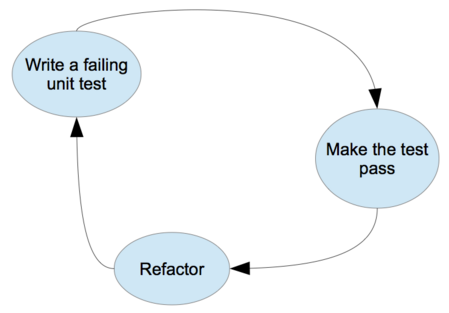
\includegraphics[height=40mm]{/home/elf/PersonalProjects/UnitTestTalk/figures/tddCycle.png}\hspace{5mm}
            };
        \end{tikzpicture}
    \end{center}
\end{frame}

\begin{frame}{Test Driven Development} 
    \begin{itemize}
        \item Rapida y continua retro-alimentacion
        \item TDD abilita refactoring
        \item Lecciones aprendidas, experiencias ganadas no se pierden, quedan en los tests
    \end{itemize}
\end{frame}

\begin{frame}{Test Driven Development} 
    \begin{itemize}
        \item Esto trae consigo desarrollo de software incremental e iterativo
        \item El codigo final generalmente esta bien disenado y 
            \textcolor{red}{tiene tests unitarios!!!!}
        \item No es la respuesta a todos los problemas en desarrollo de software, pero
            definitivamente una mejor al hack, hack, hack and fix
    \end{itemize}
\end{frame}


\end{document}
